\subsection{Segmentation}
\subsubsection{Felzenszwalb's method}
\begin{figure}[htb!]
\begin{subfigure}{.3\textwidth}

\includegraphics[width=\textwidth]{images/rufy_d.png}
\caption{Before preprocessing.}
\end{subfigure}
\begin{subfigure}{.3\textwidth}

\includegraphics[width=\textwidth]{images/luffyK100.png}
\caption{With $K = 100$.}
\label{fig:smallKSegmentation}
\end{subfigure}
\begin{subfigure}{.3\textwidth}
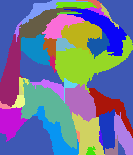
\includegraphics[width=\textwidth]{images/luffyK1000.png}
\caption{With $K = 1000$.}
\label{fig:largeKSegmentation}
\end{subfigure}
\caption{Segmentation results with Felzenszwalb's method, with a small $k$ and a larger $k$.}
\end{figure}

The segmentation method by P. F. Felzenszwalb and D. P. Huttenlocher, described in detail in \cite{felzenszwalb2004efficient}, is an efficient graph-based segmentation method for color images.

\paragraph{The method} Let $I$ be a color image. The algorithm considers a graph $G = (V,E)$ defined on the set of pixels of I with weight function $w$ measuring dissimilarity between pixels. Let $n$ be the number of vertices and $m$ the number of edges of $G$. The pseudo code of the algorithm is given in \autoref{alg:felzenszwalb}, where $MInt : S \times S \rightarrow \mathbb{R}^+$ for some segmentation $S$ is defined by:
\[
MInt(C_1, C_2) = \min(Int(C_1) + \tau(C_1), Int(C_2) + \tau(C_2))
\]
$\tau(C) = \frac{k}{|C|}$ is a threshold function for a scale parameter $k$, and $Int(C)$ measure the internal difference of a component $C$, defined by
the largest weight of the minimum spanning tree of $C$:
\[
Int(C) = \max_{\{u,v\} \in MST(C, E)} w(u,v)
\]

\begin{algorithm}
\caption{Felzenszwalb's segmentation algorithm}
\label{alg:felzenszwalb}

\begin{algorithmic}[1]
\Function{Felzenszwalb}{$G = (V, E)$}
\State Sort $E$ into $\pi = (o_1, ..., o_m)$ by ascending edge weights
\State Initialize $S_0$ with each vertex in its own component
\For{$q \gets 1$ to $m$}
\State Let $\{u,v\} = o_q$ the $q^{th}$ edge in the ordering
\State Let $C_u$ and $C_v$ the components containing $u$ and $v$ in $S_{q-1}$
\If{$C_u \neq C_v$ and $w(u,v) \leq MInt(C_u, C_v)$}
\State $S_q$ is obtained by merging $C_u$ and $C_v$ in $S_{q-1}$
\Else
\State $S_q$ is just $S_{q-1}$
\EndIf
\EndFor
\Return $S_m$
\EndFunction
\end{algorithmic}
\end{algorithm}

\paragraph{Theoretical justification} The authors show that this algorithm results in a segmentation which is neither too coarse nor too fine, according to a precise notion of boundary between segments. This is interesting for animation character images, which are characterized by large areas of homogeneous color, which this algorithm capture reasonably well.

\paragraph{Implementation} The algorithm can be implemented to run very efficiently. Using a disjoint set forest data structure for the segmentation allows the $Find$ and $Union$ operation to be performed in amortized $O(\alpha(n))$ time where $\alpha$ is the inverse of the Ackermann function, and computing $MInt$ between each iteration can be done in constant $O(1)$ time. With an adjacency list data structure for the graph $G$, it is easy to list all edges in $O(m)$ time. This makes clear that the time behavior of the algorithm is dominated by the initial sorting of edges, which can be computed in $O(mlog(m))$ time using an optimal comparison sort like merge sort.

The authors study the case where $G$ is an $8$-connected graph and where it is a variation on the $K$-nearest-neighbor graph\footnotemark
\footnotetext{
While a non-mutual $K$-nearest neighbor graph is not necessarily sparse, the authors assert that it is in their paper. As their graph construction is also not made explicit in the paper, and their source code only include an $8$-connected graph, we proceed under the optimistic assumption that the authors use a variation on the $K$-nearest-neighbor graph which is actually sparse.
}
 in $(x, y, r, g, b)$ feature space. Since both classes of graphs are sparse - the number of edges is within a constant factor of the number of vertices - this makes the time complexity of the algorithm $O(nlog(n))$.

\paragraph{Results and analysis} Although this algorithm is efficient, it suffers from a few drawbacks. The method as described above tends to create many very small components, which can be solved by a post-processing step greedily merging components smaller than a threshold. It also tends to produce segments of similar size, which in the case of animation character image is not desirable. It produces either an oversegmentation where large segments are separated in many small ones (\autoref{fig:smallKSegmentation}), or an undersegmentation where smaller segments are incorrectly merged into larger ones (\autoref{fig:largeKSegmentation}).

\subsubsection{Spectral segmentation and clustering algorithms}

\subsubsection{Felzenszwalb's method with hue-based segment merging}
